\documentclass[11pt]{article}

\usepackage[utf8]{inputenc} % Character encoding
\usepackage[T1]{fontenc}    % Large font encoding
\usepackage{lmodern}        % Latin modern font

\usepackage{float}
\usepackage{graphicx}
\usepackage{hyperref}

\usepackage{listings}	   % Code insertion
\lstdefinestyle{customstyle}{
    basicstyle=\footnotesize,
    breakatwhitespace=false,         
    breaklines=true,                 
    captionpos=b,                    
    keepspaces=true,                                                                                       
    tabsize=4,
    frame=single
}
\lstset{style=customstyle}	

\title{Projet Système de feux tricolores}
\author{Adrien Garandel \and Bao Ran \and Franck Boncler \and Jérémy Bardon}

\begin{document}

\maketitle
\tableofcontents
\newpage

%%%%%%%%%%%%%%%%%%%%%%%%%%%%%%%%%%%%%%%%%%%%
\section{Partie 1 - Deux feux synchronisés}
%%%%%%%%%%%%%%%%%%%%%%%%%%%%%%%%%%%%%%%%%%%%
Dans cette partie, on s'intéresse à la synchronisation de deux feux tricolores. On utile pour cela des réseaux de Pétri et le logiciel Roméo.

%%%%%%%%%%%%%%%%%%%%%%%
\subsection{Questions 1 et 2}
%%%%%%%%%%%%%%%%%%%%%%%
Feux non synchronisés et non temporises

\begin{figure}[H]
	\centering
	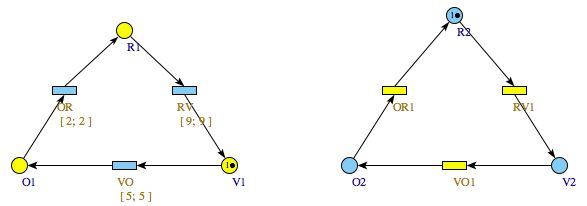
\includegraphics[width=1\textwidth]{ressources/part1/Q2.png}
	\caption{Réseau de Pétri, feux non synchronisés}
\end{figure}

Chaque feu est identique et dispose de trois places suivant les trois couleurs qu'un feu de circulation tricolore peut prendre: Rouge, Orange et Vert.

%%%%%%%%%%%%%%%%%%%%%%%
\subsection{Question 3}
%%%%%%%%%%%%%%%%%%%%%%%

\href{https://github.com/masters-info-nantes/hong-cheng-lv/blob/master/ressources/part1/Q3-FeuxSynchro.xml}{Feux
synchronisés et non temporises}

\begin{figure}[H]
	\centering
	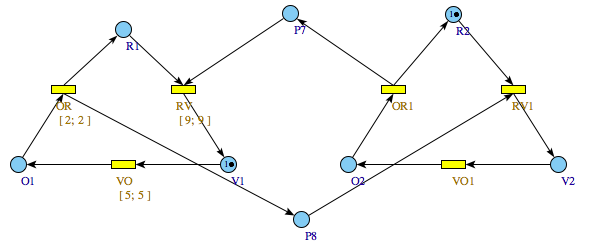
\includegraphics[width=1\textwidth]{ressources/part1/Q3.png}
	\caption{Réseau de Pétri, feux synchronisés}
\end{figure}

Dans le cas réel, les feux de circulation sont synchronisés. En effet, lorsqu'un premier feu est Vert, le second est Rouge. Puis le premier feu passe alternativement au Orange puis au Rouge tandis qu'ensuite le second feu devient Vert.

Pour respecter ce cahier des charges, nous avons ajouté deux places entre les deux feux. Alors, lorsqu'un feu devient Vert, il empêche l'autre de devenir Vert puis le libère une fois qu'il est passé à l'Orange puis au Rouge.
 
%%%%%%%%%%%%%%%%%%%%%%%
\subsection{Question 4}
%%%%%%%%%%%%%%%%%%%%%%%

Un graphe de marquage permet de montrer les différentes executions possibles de notre système de réseaux de Pétri.

\begin{figure}[H]
	\centering
	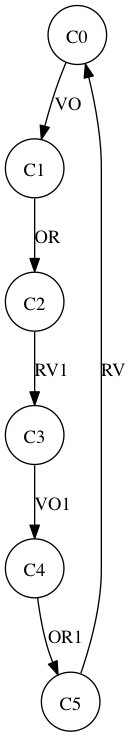
\includegraphics[scale=0.5]{ressources/part1/traitement-question4/graphe.png}
	\caption{Graphe de marquage des feux synchronisés}
\end{figure}

On constate que l'execution de notre système est linéaire. Cela signifie qu'il existe une seule execution, ainsi prouver que celle-ci est correcte revient à prouver que le système entier est correct.

%%%%%%%%%%%%%%%%%%%%%%%
\subsection{Question 5 et 6}
%%%%%%%%%%%%%%%%%%%%%%%

Vérification des propriétés de sureté de vivacité du système de feux synchronisés.

\begin{itemize}
	\item Il y a toujours au minimum un feu rouge (sureté)
\begin{verbatim}
AG[0, inf](M(R1) + M(R2) >= 1)	
\end{verbatim}

	\item Un feu passe au moins une fois au vert (non bloqué)
\begin{verbatim}
AG[0, inf](M(V2) = 1)	
\end{verbatim}

	\item Les feux ne se bloquent pas entre eux
\begin{verbatim}
AG[0, inf](M(R1) + M(P7)) # P7 = place intermédiaire	
\end{verbatim}
\end{itemize}

%%%%%%%%%%%%%%%%%%%%%%%%%%%%%%%%%%%%%%%%%%%%
\section{Partie 2 - Deux feux temporises}
%%%%%%%%%%%%%%%%%%%%%%%%%%%%%%%%%%%%%%%%%%%%
La partie précédente expose un système de feux synchronisés mais non temporises. En effet, ans la réalité les feux restent temps donné dans leurs états. Nous proposons alors un système de feux temporises sous la forme d'automates à états finis modélisés avec le logiciel Uppaal.

%%%%%%%%%%%%%%%%%%%%%%%
\subsection{Question 7}
%%%%%%%%%%%%%%%%%%%%%%%

\href{https://github.com/masters-info-nantes/hong-cheng-lv/blob/master/ressources/part2/Q7-FeuxTemporises.xml}{Feux temporisés sans synchronisation}

\begin{figure}[H]
	\centering
	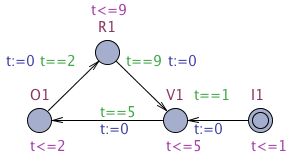
\includegraphics{ressources/part2/Q7-1.png}
	\caption{Automate du feu commençant en Vert}
\end{figure}

\begin{figure}[H]
	\centering
	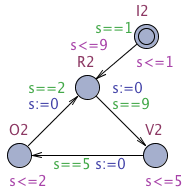
\includegraphics{ressources/part2/Q7-2.png}
	\caption{Automate du feu commençant en Rouge}
\end{figure}

Pour les deux feux, il est nécessaire d'ajouter une place initiale pour indiquer l'état initial de chacun des feux. Ce premier état attend une seconde car sinon les automates ne démarrent pas en même temps et on observerait une désynchronisation des feux.


\subsection*{Validation des propriétés de sureté de vivacité du système de feux temporises.}

\begin{itemize}
	\item Toujours au moins un feu rouge
\begin{verbatim}
A[](feu1.R1 or feu2.R2 or feu1.I1 or feu2.I2)
\end{verbatim}

	\item Les deux feux atteignent leur état le plus éloigné, ils ne sont pas bloqués par le temps
\begin{verbatim}
E<>(feu1.R1 and feu2.02)	
\end{verbatim}

	\item Pas de blocage
\begin{verbatim}
E<> deadlock
\end{verbatim}

\end{itemize}

%%%%%%%%%%%%%%%%%%%%%%%
\subsection{Question 8}
%%%%%%%%%%%%%%%%%%%%%%%

Afin de controller au mieux le système, cette solution propose l'utilisation d'un controleur. Cet élément est chargé de faire évoluer les états des feux. 

\begin{figure}[H]
	\centering
	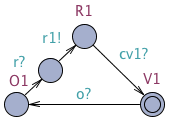
\includegraphics{ressources/part2/Q8-1.png}
	\caption{Automate du feu commençant en Vert}
\end{figure}

\begin{figure}[H]
	\centering
	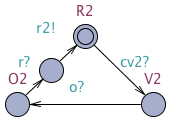
\includegraphics{ressources/part2/Q8-2.png}
	\caption{Automate du feu commençant en Rouge}
\end{figure}

\begin{figure}[H]
	\centering
	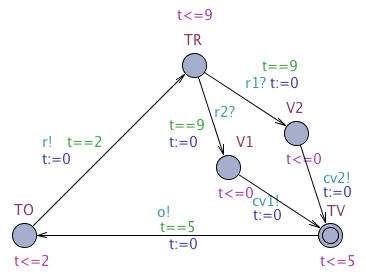
\includegraphics[width=1\textwidth]{ressources/part2/Q8-3.png}
	\caption{Contrôleur des feux}
\end{figure}

Les feux ne sont pas temporises mais il a y toujours un feu Rouge et un feu Vert au démarrage du système. En effet, c'est le rôle du contrôleur qui temporise et commande les feux à travers une synchronisation par signaux. 

Le contrôleur allume alors alternativement le premier et le second feu tout en prenant en compte le temps pendant lequel un feu doit rester dans un état donné.

\subsection*{Vérification des propriétés de sureté de vivacité du système de feux synchronisés}

\begin{itemize}
	\item Toujours au moins un feu rouge
\begin{verbatim}
A[](feu1.R1 or feu2.R2)
\end{verbatim}

	\item Les deux feux atteignent leur état le plus éloigné, ils ne sont pas bloqués par le temps
\begin{verbatim}
E<>(feu1.R1 and feu2.O2)
\end{verbatim}

	\item Pas de deadlock
\begin{verbatim}
E<> deadlock
\end{verbatim}

\end{itemize}

%%%%%%%%%%%%%%%%%%%%%%%%%%%%%%%%%%%%%%%%%%%%
\section{Partie 3 - Carrefour en T}
%%%%%%%%%%%%%%%%%%%%%%%%%%%%%%%%%%%%%%%%%%%%
Après avoir étudier des systèmes représentant la synchronisation de deux de circulation sur une route, nous allons nous intéresser à un carrefour en T.

Comme dans le premier cas, il y a une route principale avec deux feux tricolores. On ajoute ici une route mineure sur le côté. Dans un cas normal, le feux de la route mineure est Rouge mais lorsque des voitures sont captés il passe au Vert.

%%%%%%%%%%%%%%%%%%%%%%%
\subsection{Question 9}
%%%%%%%%%%%%%%%%%%%%%%%

Dans cette première version de notre système de feux, il n'y a pas de contraintes de temps.

% expliquer r2c

\begin{itemize}
	\item Les 2 feux de la grande route sont considérés comme un seul
	\item Processus qui régule l'arrivée des voitures dans la petite rue
\end{itemize}

\begin{figure}[H]
	\centering
	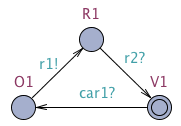
\includegraphics{ressources/part3/Q9-1.png}
	\caption{Automate du feu de la route majeure}
\end{figure}

Le feu de la route principale passe du Vert au Orange puis au Rouge lorsqu'un véhicule arrive sur la route mineure. Il attend alors qu'il n'y ai plus de voiture sur la route mineure pour repasser au Vert.

\begin{figure}[H]
	\centering
	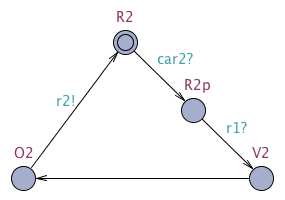
\includegraphics{ressources/part3/Q9-2.png}
	\caption{Automate du feu de la route mineure}
\end{figure}

Par défaut Rouge, le feu de la route mineure passe au Vert si une voiture est capté et une fois que les feux de la route principale sont Rouges.

\begin{figure}[H]
	\centering
	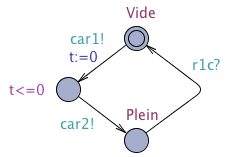
\includegraphics{ressources/part3/Q9-3.png}
	\caption{Automate de l'arrivée des véhicules sur la route mineure (capteur)}
\end{figure}

Cet automate régule l'arrivée de voiture sur la route mineure. Il détecte alors une voiture toutes les 50 tocs d'horloges. Le signal \emph{r2c} permet de d'assurer que la voiture détectée sur la route mineure soit bien passée avant que le feu repasse au Vert.

%%%%%%%%%%%%%%%%%%%%%%%
\subsection{Question 10}
%%%%%%%%%%%%%%%%%%%%%%%

A notre système de feux sur un carrefour en T, nous ajoutons ici des contraintes de temps notamment sur le temps pendant lequel chaque feu doit rester Vert.

\begin{itemize}
	\item Petite rue verte 30 secondes
	\item Dans un cycle, la grande route est Verte au moins 30 secondes
	\item Délai de 1 seconde entre chaque changement de couleur
	\item Chaque feu reste orange pendant 5 secondes
\end{itemize}

Les signaux \emph{r1} et \emph{r2} permettent d'obliger qu'un des feux soit rouge à n'importe quel moment.

\begin{figure}[H]
	\centering
	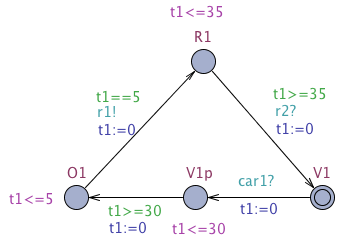
\includegraphics{ressources/part3/Q10-1.png}
	\caption{Automate du feu de la route majeure}
\end{figure}

La grande route attend qu'une voiture arrive sur la petite route pour passer à l'Orange une fois qu'il a été au moins 30 secondes Vert depuis le début.

Avant de repasser au Vert une fois Rouge, le feu de la route majeure attend que celui de la route mineure soit passé au Rouge.

\begin{figure}[H]
	\centering
	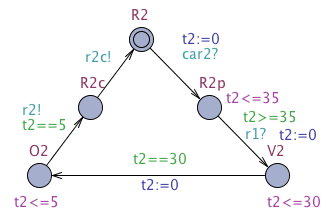
\includegraphics{ressources/part3/Q10-2.png}
	\caption{Automate du feu de la route mineure}
\end{figure}

Pour passer au vert, le feu de la route mineure doit attendre de capter une voiture mais aussi que le feu de la route majeure soit Rouge.

\begin{figure}[H]
	\centering
	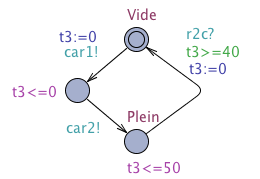
\includegraphics{ressources/part3/Q10-3.png}
	\caption{Automate de l'arrivée des véhicules sur la route mineure (capteur)}
\end{figure}

%%%%%%%%%%%%%%%%%%%%%%%
\subsection{Question 11}
%%%%%%%%%%%%%%%%%%%%%%%

%%%%%%%%%%%
\subsubsection{Validations question 9}
%%%%%%%%%%%

\begin{itemize}
	\item Toujours au moins un feu rouge
\begin{verbatim}
A[](Major.R1 or Minor.R2 or Minor.R2p or Minor.R2v)
\end{verbatim}
	
	\item Lorsque le feu de la petite route passe au vert, la voiture qui attend passe
\begin{verbatim}
E<>(Car.Vide and Minor.V2)
\end{verbatim}
	
	\item Les deux feux atteignent leur état le plus éloigné, ils ne sont pas bloqués par le temps
\begin{verbatim}
E<>(Major.R1 and Minor.O2)
\end{verbatim}
	
	\item Pas de deadlock
\begin{verbatim}
E<> deadlock
\end{verbatim}

\end{itemize}

%%%%%%%%%%%
\subsubsection{Validations question 10}
%%%%%%%%%%%

\begin{itemize}
	\item Toujours au moins un feu rouge
\begin{verbatim}
A[](Major.R1 or Minor.R2 or Minor.R2p or Minor.R2c)
\end{verbatim}

	\item Les deux feux atteignent leur état le plus éloigné, ils ne sont pas bloqués par le temps
\begin{verbatim}
E<>(Major.R1 and Minor.O2)
\end{verbatim}

	\item Pas de deadlock
\begin{verbatim}
E<> deadlock
\end{verbatim}
\end{itemize}

%%%%%%%%%%%%%%%%%%%%%%%%%%%%%%%%%%%%%%%%%%%%
\section{Implémentation}
%%%%%%%%%%%%%%%%%%%%%%%%%%%%%%%%%%%%%%%%%%%%

\end{document}
